\section{Common Source Amplifier}

\subsection{Procedure}

The input source of the circuit in figure \ref{fig:circuit} is set to a $50 mVpp$ sinusoid with a $1 kHz$ frequency.
The sinusoidal input signal is offset by $2.5 V$ DC, after making necessary adjustments to the bias point found in the previous portion of the experiment.
The oscilloscope is set to measure time-domain signals to find the amplitude of the output signal.
The gain of the amplifier is then calculated from the measurements and is compared to the theoretical result.

\FloatBarrier

\subsection{Results}

The DC bias current $I_D$ of the amplifier is found using the values found for $V_{DD}$, $V_{out}$, and $R$ in the previous section.

\FloatBarrier

\begin{equation}
	\label{eq:bias_current}
	I_D = \frac{V_{DD}-V_{out}}{R} = \frac{10 V - 4.875 V}{295.3 \Omega} = 17.4 mA
\end{equation}

\FloatBarrier

The theoretical transconductance $g_m$ of the amplifier can be calculated using the given transconductance parameter $k_n$ of $80 mA/V$ and the $I_D$ found in equation \ref{eq:bias_current}.

\FloatBarrier

\begin{equation}
	\label{eq:g_m}
	g_m = \sqrt{2k_nI_D} = \sqrt{2(80 mA/V^2)(17.4 mA)} = 52.8 mA/V
\end{equation}

\FloatBarrier

Using the small signal model for the common source amplifier and using KCL at the drain node, the equation to find the theoretical open loop gain $A_{vo}$ is found.

\FloatBarrier

\begin{equation}
	\label{eq:ss_kcl}
	-g_mV_{in} = \frac{V_{out}}{R} \rightarrow A_{vo} = \frac{V_{out}}{V{in}} = -g_mR
\end{equation}

\FloatBarrier

The theoretical open loop gain $A_{vo}$ of the amplifier can then be found using the transconductance $g_m$ in equation \ref{eq:g_m}.

\FloatBarrier

\begin{equation}
	\label{eq:theoretical_gain}
	A_{vo} = -g_mR = -(52.8 mA/V)(295.3 \Omega) = -15.6 V/V \\
\end{equation}

\begin{equation}
	\label{eq:theoretical_gain_db}
        gain \ in \ dB = 20 log(|-15.6|) = 23.9 dB
\end{equation}

\FloatBarrier

The following input and output voltages are measured using the oscilloscope.

\FloatBarrier

\begin{figure}[h!]
	\centering
		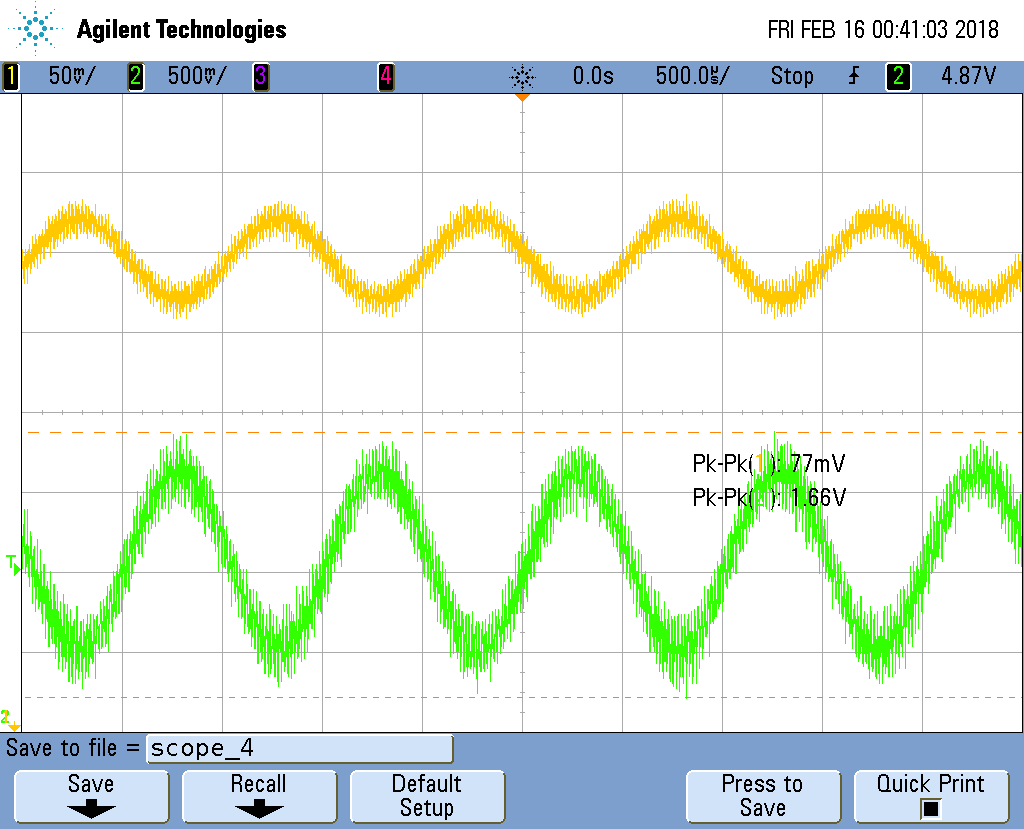
\includegraphics[scale=0.35]{./images/scope_4.png}
		\caption{Input and Output Voltages Measured}
		\label{fig:measured_vin_vout}
\end{figure}

\FloatBarrier

From figure \ref{fig:measured_vin_vout}, the measured peak-to-peak amplitudes of $V_{in}$ and $V_{out}$ are $77 mVpp$ and $-1.66 Vpp$, respectively.
The peak-to-peak amplitude of the input signal measured from the oscilloscope will be used instead of the ideal $50 mVpp$ value set on the function generator because the signals measured on the oscilloscope account for noise, loading effects, and other nonidealities in the waveforms.
The values found in figure \ref{fig:measured_vin_vout} are used to calculate the measured gain of the amplifier.

\FloatBarrier

\begin{equation}
	\label{eq:measured_gain}
	A_{vo} = - \frac{V_{out}}{V_{in}} = \frac{-1.66 V}{0.077 V} = -21.6 V/V
\end{equation}

\begin{equation}
	\label{eq:measured_gain_db}
	gain \ in \ dB = 20 log(|-21.6|) = 26.7 dB
\end{equation}

\FloatBarrier

The percent error of the measured and theoretical gains are found using the following equation:

\begin{equation}
	\label{eq:error}
	error \ in \ amplitude \ gain = - |\frac{(-21.6) - (-15.6)}{-15.6}| * 100\% = 38\%
\end{equation}

\begin{equation}
	\label{eq:error_db}
        error \ in \ dB \ gain = - |\frac{26.7 dB - 23.9 dB}{23.9 dB}| * 100\% = 12\%
\end{equation}

 The measured gain and theoretical gain are in the same order of magnitude and the measured gain in dB is close to the theoretical value.
 Therefore, the measured results show that the theoretical model of the MOSFET is adequate in predicting experimental behavior.
